\chapter{PRODUCED TEST AUTOMATION SYSTEM}\label{chapter:produced_test_automation_system}
In this chapter, the final plans for the system are presented. The first section will present management-related subjects, and the second will concentrate on more technical matters.

\section{Management}
This section presents the Hubshare test automation system's management plans. First, the overall test automation process will be presented. After the whole picture, the competencies of different stakeholders will be discussed. In the third section, some test automation conventions are described. Finally, the introduction of the new test automation system will be presented.

\subsection{Test automation process}
As shown in the \autoref{fig:process_flow_of_new_test_cases}, test automation cases follow the normal Scrum process shortly described in the \autoref{subsection:test_automation_daily_activities}. Initially, new test automation cases are developed by a developer. After the developer thinks that the new test cases are good enough, the test cases will be reviewed by another developer. New test automation cases will be declared ready if the review is successful. After the sprint is over, a sprint review will be held, verifying that the new test automation cases are sufficient. If so, cases will become officially part of the test automation case repository.

\begin{figure}
	\centering
	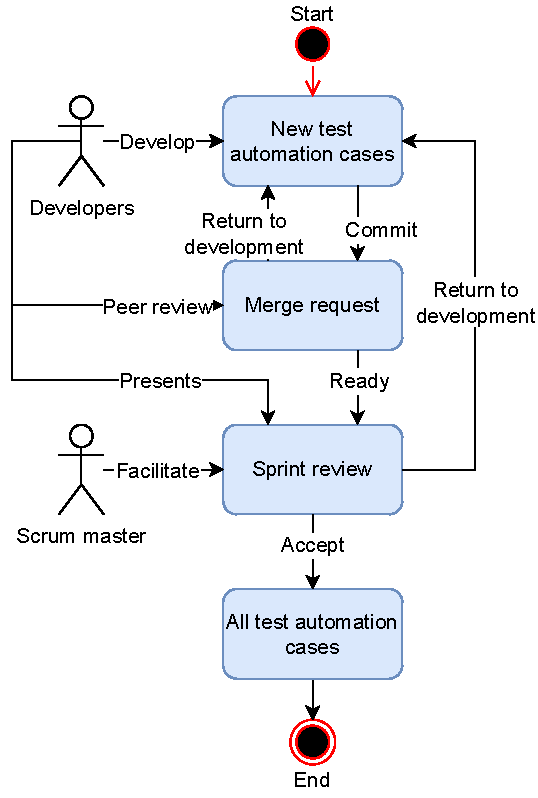
\includegraphics[width=0.6\textwidth]{New_test_cases_process_flow}
	\caption{Process flow of the new test automation cases}
	\label{fig:process_flow_of_new_test_cases}
\end{figure}

From the code perspective, new test automation case production works slightly differently. As can be seen from the \autoref{fig:code_flow_of_new_test_cases}, new test automation cases are produced together with the code. In the \autoref{fig:process_flow_of_new_test_cases}, the production code follows the same path as the test automation code, but in that specific figure, the production code is not specially mentioned. After the test automation cases and the production code has been developed, new code will be committed to the \glsfirst{mr}. \gls{mr} will be peer-reviewed by a fellow developer, and if the reviewer approves the \gls{mr}, new test automation cases will be merged into the integration branch. So basically, the new test automation cases will be used immediately, even though they are entirely accepted to be part of the test automation case collection only after the sprint review has been kept.

In the \autoref{fig:code_flow_of_new_test_cases}, it is also notable that developers develop mainly only new test cases. Development of the test automation framework marked with green in the \autoref{fig:code_flow_of_new_test_cases} is mainly done by the separate test automation team as suggested by the literature and mentioned in the \autoref{subsection:test_automation_roles}. Another notable fact in the diagram is that the new test automation cases' development order and the code are not defined. As stated in the \autoref{subsection:management_key_findings}, this is because \gls{tdd} based development would be too much for the developers that are not so familiar with the test automation.

\begin{figure}
	\centering
	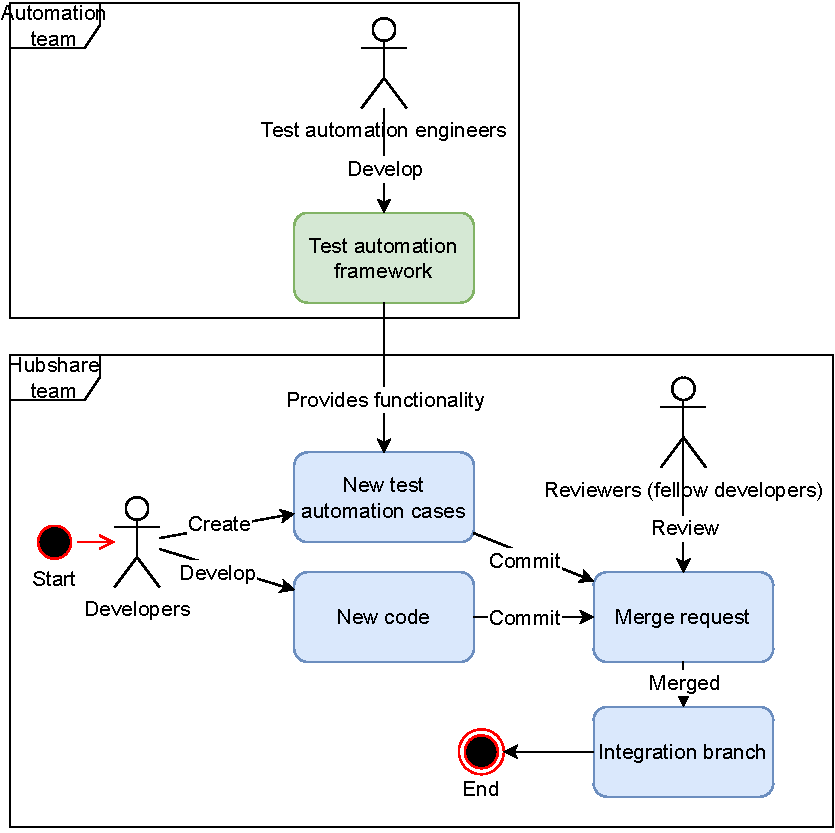
\includegraphics[width=0.7\textwidth]{New_test_cases_code_flow}
	\caption{Code flow of the new test automation cases}
	\label{fig:code_flow_of_new_test_cases}
\end{figure}

Even though it is not emphasised in either of the figures, passing all of the prior test automation cases is a hard prerequisite before \gls{mr} can be accepted. The passing of the test cases is an essential rule from the test automation perspective. Without such a requirement, the usefulness of the test automation would be questionable because the results would not be used. In addition, the quality of the test automation would slowly start degrading because the test cases would not be actively checked and repaired as happened with the prior attempts mentioned in the \autoref{section:case_new_test_automation_system_for_hubshare}. 100\% passing of the test cases has also been seen as a necessity in the literature because if the test cases were left failing, it would soon become unclear who should repair the failing cases \cite{beck2000extreme}.
\FloatBarrier

\subsection{Test automation responsibilities}
Test automation responsibilities are divided between management, developers, team's \gls{qa} engineer and test automation teams. Based on the \autoref{subsection:test_automation_roles} details, management should ensure sufficient resources and support for the test automation efforts. Management should also enforce defined test automation processes because otherwise, there is a possibility that, for example, developers will begin slacking off with the test automation activities.

Developers' have many practical responsibilities related to test automation. The developer's primary responsibility is to write new test automation cases. In addition, developers review other developers' \glspl{mr} and, for example, fix test automation cases if the test cases become broken during an \gls{us} development. Developers are primary creators of the test automation cases because they have the best knowledge of the \gls{us} and sufficient technical knowledge to implement new test automation cases appropriately. This approach is also recommended in the literature as was mentioned in the \autoref{subsection:test_automation_roles}. Additionally, developers own the automation cases they created and are responsible for fixing the potential problems with the test cases. The importance of ownership was mentioned in the \autoref{subsection:management_key_findings}.

The team's \gls{qa} engineer's responsibility is to assist developers in writing better test automation cases. For example, \gls{qa} can advise what developers could test and which way the testing could be done. Additionally, \gls{qa} can help with the reviews of the \glspl{mr} by providing feedback about the quality and coverage of the implemented test cases. As mentioned in the \autoref{subsection:quality_assurance}, \gls{qa}'s second opinion is valuable because of the different mindset compared to developers.

The test automation team is responsible for improving the framework part of the test automation system. Improving is done by adding new features to the framework based on the developers' wishes and requests. The test automation team is also responsible for the environments and essential monitoring of the test automation system. If there are any environment-related issues, the test automation team should fix those problems. This approach was also chosen based on the literature recommendations mentioned in the \autoref{subsection:test_automation_roles}.

\subsection{Test automation conventions}\label{subsection:test_automation_conventions}
Under this subsection, various test automation conventions are explained. These conventions are only minor details, but they significantly impact the project's success when combined. Without these details, produced test automation system could have enormous problems in the future.

One of the defined conventions is the 80\% line coverage target. Target states that the 80\% coverage would be desirable on all test levels for the newly produced user stories. However, the target is not absolute and is instead only indicative because it is understood that the target can be too hard to reach feasibly in some scenarios. For example, testing all error scenarios using the system-level testing framework would not be wise. Some coverage target was still selected to guide the test automation cases' development and utilise collected coverage metrics that were part of the test automation framework's requirements available in the \autoref{appendix:projects_requirements}.

During planning, it was discovered that line coverage might not be the most suitable metric for all testing levels. For example, it would have been nice to measure the coverage of different functionalities at the system testing level instead of calculating the line coverage. However, alternative calculation methods were technically challenging, and the line coverage method was still used on all testing levels.

Method name-should-when naming scheme was selected as a naming convention for the test automation cases. The scheme defines that the test case name should start with the method name, continue with the clause that describes what the test does and end with the clause that lists the conditions for the test case. The naming convention was defined because, in the literature, it is stated that any naming convention can be selected as long as some are decided so that test case names will be consistent \cite{stefanovskyi2019unit}. Method name-should-when convention was explicitly selected because it seemed to work best for the test case names that were sketched before the final naming convention was selected. Overall good test case names are essential because in the future, when there will be thousands of test cases, it can be hard to understand quickly what the test case is about if the name is unclear or even find the method from the source code based on the \gls{ci} log.

One special convention was also defined for the assertions. During interviews, it was mentioned multiple times that easy-to-understand assertions are essential for good test automation cases. It was decided that all assertions must include custom failure messages to ensure that all assertions would be as easy to understand as possible. Custom failure messages should speed up the future diagnosis of failing test cases when developers can immediately see what went wrong with the specific test case.

\subsection{Test automation introduction plan}\label{subsection:test_automation_introduction_plan}
The introduction plan has the following phases:
\begin{enumerate}[noitemsep]
	\item Initial education and unit test frameworks are taken into use.
	\begin{enumerate}[label*=\arabic{enumii}.,noitemsep]
		\item Overhaul of the backend unit testing framework.
		\item Implementation of the frontend unit testing framework.
		\item Education sessions about general test automation and the new frameworks.
		\item Taking unit test automation into use.
	\end{enumerate}
	\item Initial introduction of \gls{api} and component integration testing frameworks.
	\begin{enumerate}[label*=\arabic{enumii}.,noitemsep]
		\item Overhaul of the \gls{api} testing framework.
		\item Overhaul of the integration testing framework.
		\item Integration testing-related education sessions.
		\item Integration testing frameworks are taken into use.
	\end{enumerate}
	\item System testing framework.
	\begin{enumerate}[label*=\arabic{enumii}.,noitemsep]
		\item Implementation of the system testing framework.
		\item System testing-related education sessions.
		\item System testing framework is taken into use.
	\end{enumerate}
	\item Implementation of the complex cases.
\end{enumerate}

During the first phase, as seen from the introduction plan outline, initial education sessions are kept, and the unit testing framework is constructed and taken into daily use. Initial education sessions introduce and justify the existence of test automation for developers and provide sufficient technical knowledge about the produced test automation frameworks. During the construction of the unit testing frameworks, separate unit testing frameworks for the backend and frontend are implemented. Finally, the test automation practises and system is taken into daily production after the education sessions are finished and the framework is ready for use.

The integration and system testing levels' plans are similar to the unit testing plans. The most significant difference compared to unit testing is that during these phases, there will not be any additional general education sessions. Instead, the education will strictly focus on technical aspects.

During the final phase, more complex test automation scenarios will be tested. More challenging scenarios consist of test cases that require connections to external systems, such as a search engine. More complicated scenarios also include cases that require the presence of the M-Files server installation.

There were various reasons why this particular introduction plan was selected. Interestingly from the management point of view, the order was unimportant because the management's goal was to only have as good test automation frameworks as possible regardless of the implementation order. Because of that, the implementation order could be in theory selected freely.

Unit testing frameworks were decided to be implemented first because the developers writing the test automation cases in the beginning did not have excellent knowledge about the writing of the test automation cases. It was believed that the unit tests close to the code would be easiest for the developers from an educational point of view. Additionally, it was estimated that implementing the unit testing frameworks would be the most straightforward and take the shortest time. Because of this, by implementing the unit testing frameworks first, it would be possible to start the test automation activities as soon as possible.

After completing the unit testing frameworks, an overhaul of the \gls{api} testing framework was started. Implementation of the \gls{api} testing framework was scheduled to be next because the \gls{api} testing framework was already partially implemented before. Because of that, the implementation of the framework was easier to finalise. An additional advantage of beginning with the \gls{api} testing framework is that the \gls{api}, component integration and system-level test frameworks require similar initialisation code as mentioned in the \autoref{subsection:integration_testing_architecture}. The initialisation code was easiest to be implemented based on the existing implementation. After the \gls{api} testing framework is ready, it should be easy to construct a component-level integration testing framework based on the standard initialisation code as well as the system testing framework.

After the unit and integration level testing frameworks are ready, implementing the system-level test automation framework should be straightforward based on the accumulated knowledge gathered during the previous phases. Because of that, the system-level testing framework was scheduled to be the last of the bunch. Finally, more challenging test automation cases would be implemented on top of the existing test frameworks. More demanding test automation cases were decided to be implemented last because implementing those test cases is forecasted to take a considerable amount of time. If the functionality had been implemented earlier, the test automation introduction would have slowed down. The downside of this approach is that the automation test cases that require complex functionalities are not available during the original introduction of the test automation.

\subsection{Test automation improvement plan}
Because test automation is introduced late in the product development's life cycle, a significant amount of old code exists, which should be covered with test automation cases. The straightforward approach to increase test coverage would be to create several tasks during which test automation would be improved. However, this may not be a great approach because adding these tasks to the otherwise busy schedule could be hard to justify. In addition, developers would likely soon get bored if they were forced to implement test automation cases for an extended period of time. Additionally, it would require extra effort to prioritise these tasks so that the most critical areas of the code would be covered first.

Something else needed to be invented to avoid the problems mentioned above. After planning, it was defined that improvements to the test automation coverage should be made during the bug fixes. During the bug fixing, a new test automation case should be added to verify that the bug cannot happen again. Additionally, new test automation cases should be added to the immediate vicinity of the bug and slightly further away to ensure no further bugs are present nearby. The problems with scheduling, prioritisation and developers' interest can be effectively and automatically avoided with bug-oriented test automation improvements approach.

\section{Technical}\label{section:technical}
This section describes key technical details of the test automation systems. Higher-level architectural pictures of the system are included in this section, but exact details that are insignificant to the overall architecture are omitted. The section includes three subsections, one corresponding to each testing level.

Hubshare application's immediate surroundings can be seen in the \gls{c4} context diagram in the \autoref{fig:hubshare_context_diagram}. As seen from the figure, Hubshare has many external dependencies coloured in grey and one internal dependency coloured in blue in the form of an M-Files server. Multiple dependencies increase the higher testing levels complexity because, logically, more systems require prior preparations. As mentioned earlier in the \autoref{subsection:test_automation_introduction_plan}, these external system dependencies are considered complex and will be added to the test automation system last.

\begin{figure}
	\centering
	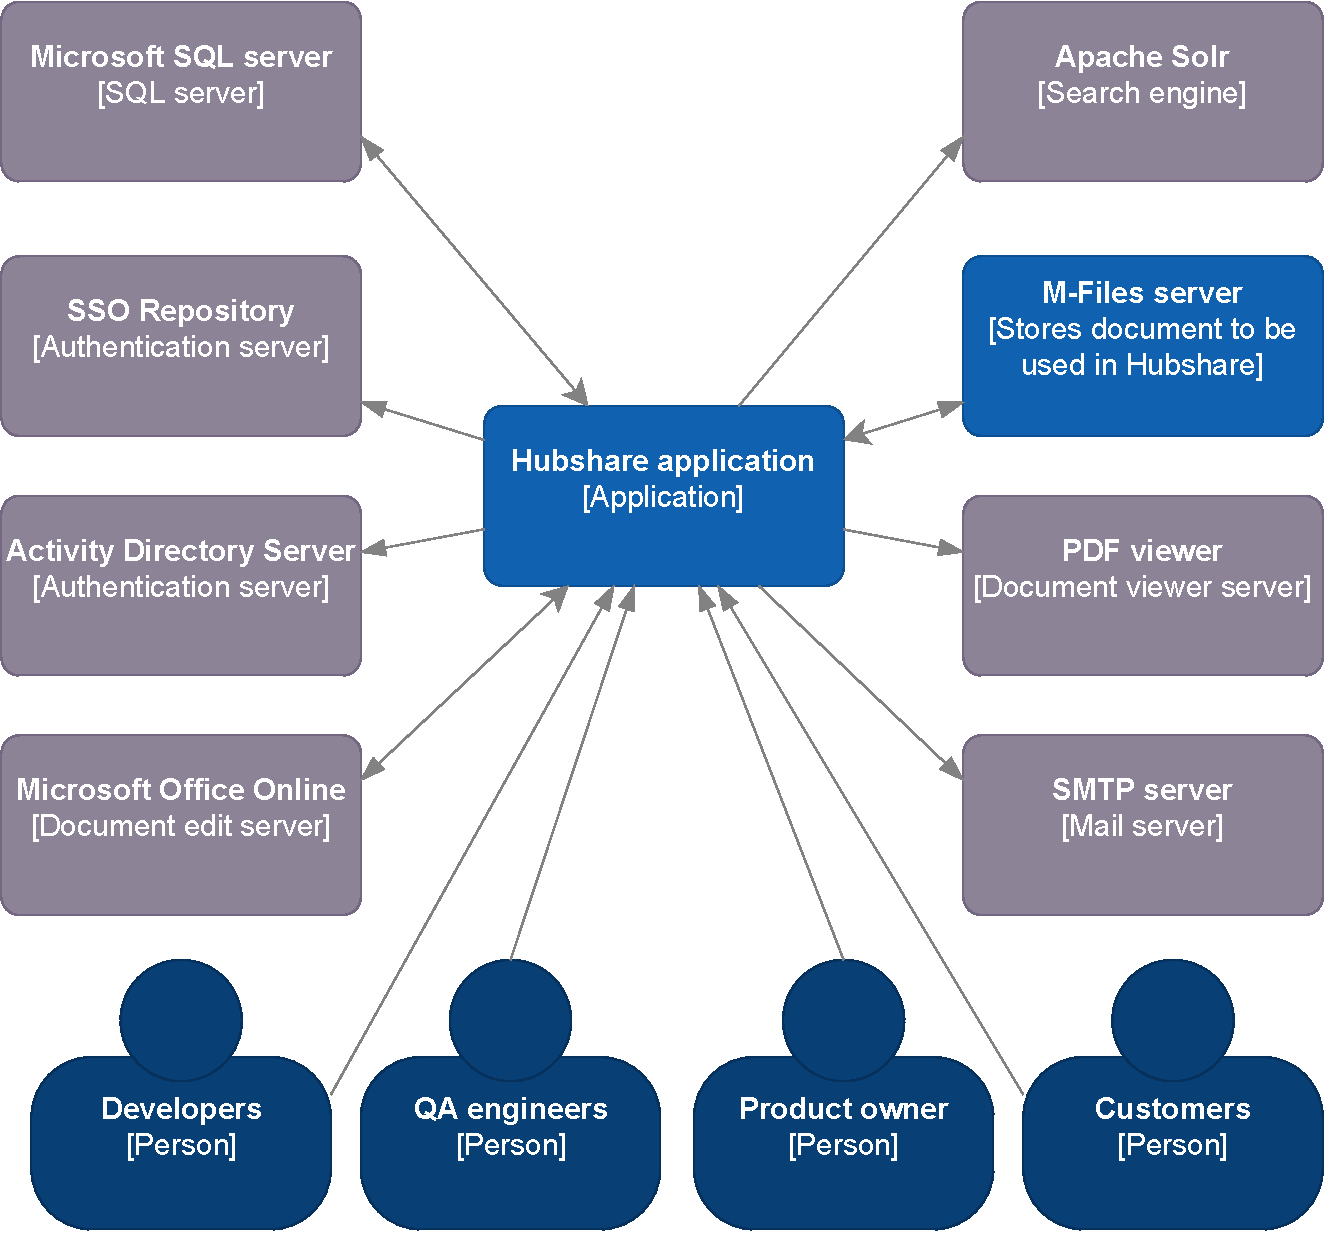
\includegraphics{Context_diagram}
	\caption{Hubshare context diagram}
	\label{fig:hubshare_context_diagram}
\end{figure}

Relations of the different overall test automation system containers are presented in the \autoref{fig:test_automation_layers}. Directly addressable systems are coloured blue, while supporting systems are coloured grey. As seen from the figure, different parts of the overall test automation system support each other, and more complex test automation layers are built atop the simpler layers. A couple of more generic support libraries were required to foster container interoperability. The most notable support library is the "Integration testing common", which contains all the necessary functionalities for setting up the Hubshare application. Its functionalities are heavily used by all the higher-level test automation systems. The higher level architecture reflects the ideas presented in the \autoref{subsection:integration_testing_architecture}.

\begin{figure}
	\centering
	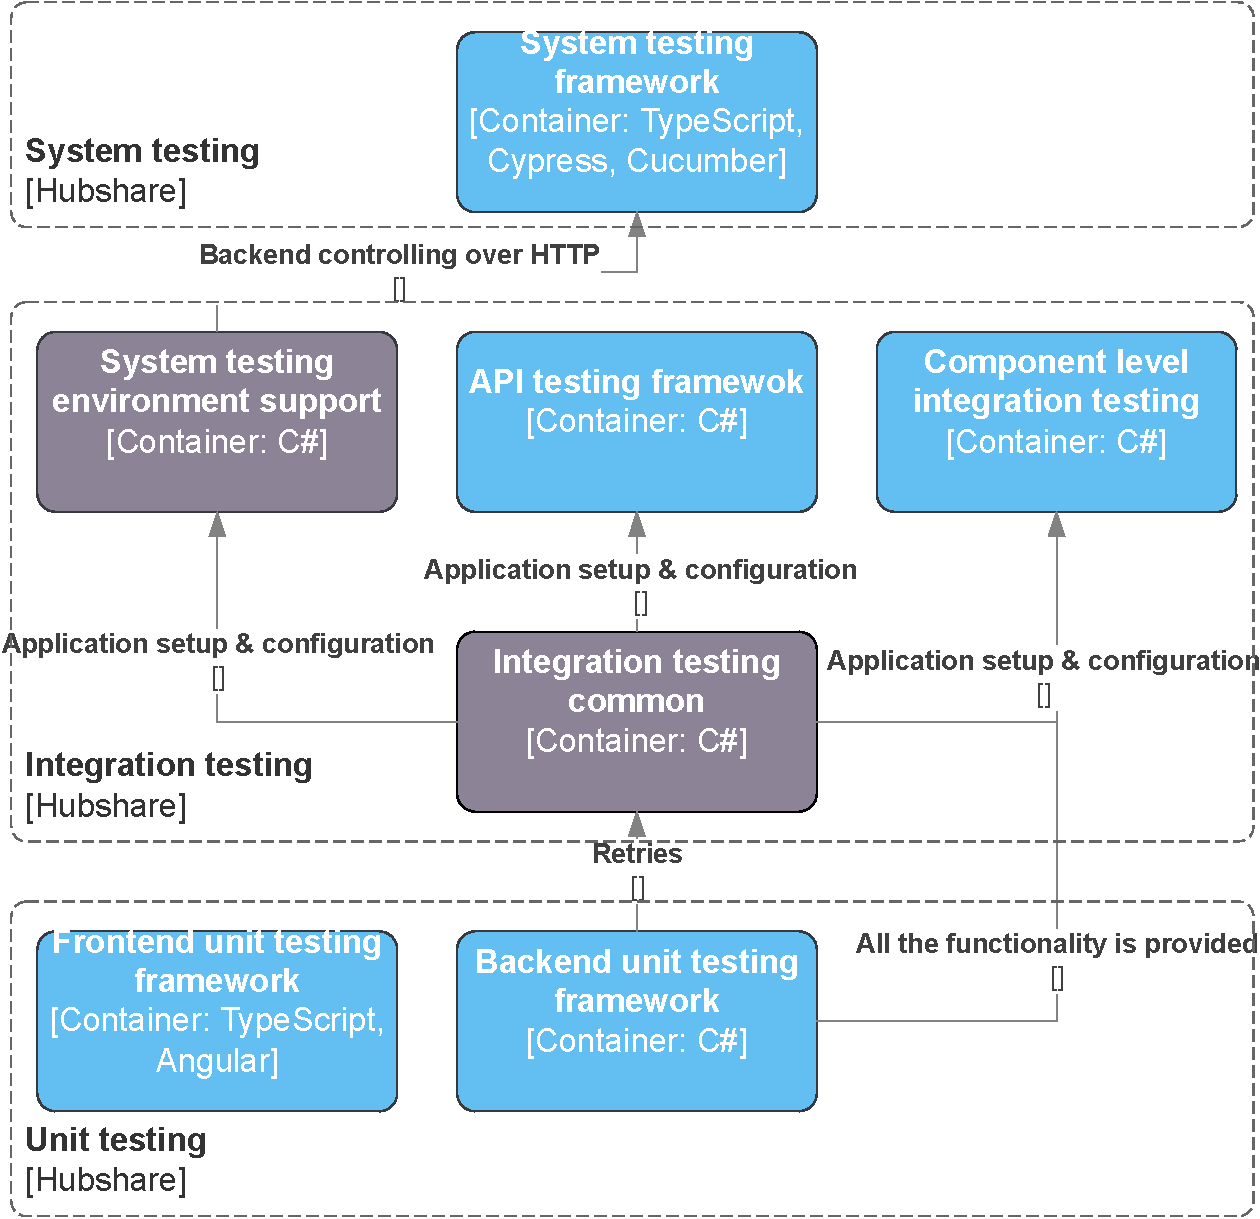
\includegraphics{Test_automation_layers}
	\caption{Test automation system container relations}
	\label{fig:test_automation_layers}
\end{figure}
\FloatBarrier

\subsection{Unit test automation}
An overview of the backend unit testing system's architecture can be seen in the \autoref{fig:backend_unit_testing_component_diagram}. The figure is divided into three different component types marked with distinctive colours. External components are grey, internally developed testing components are green and internally developed software component is blue.

There are three main externally developed components, xUnit unit testing framework, Moq mocking library and Fluent Assertions. xUnit was selected as the primary testing library mainly due to its trustworthy roots and popularity. xUnit is written by original authors of the popular unit testing library called NUnit \cite{xunit2022home}. Because the original authors had noticed mistakes in the NUnit, they created a new framework that would correct prior mistakes \cite{xunit2022why}. Even the maintainer of the C\#-language, Microsoft, seems to be endorsing the xUnit framework by mentioning the framework first in their documentation \cite{microsoft2022testing}.

\begin{figure}
	\centering
	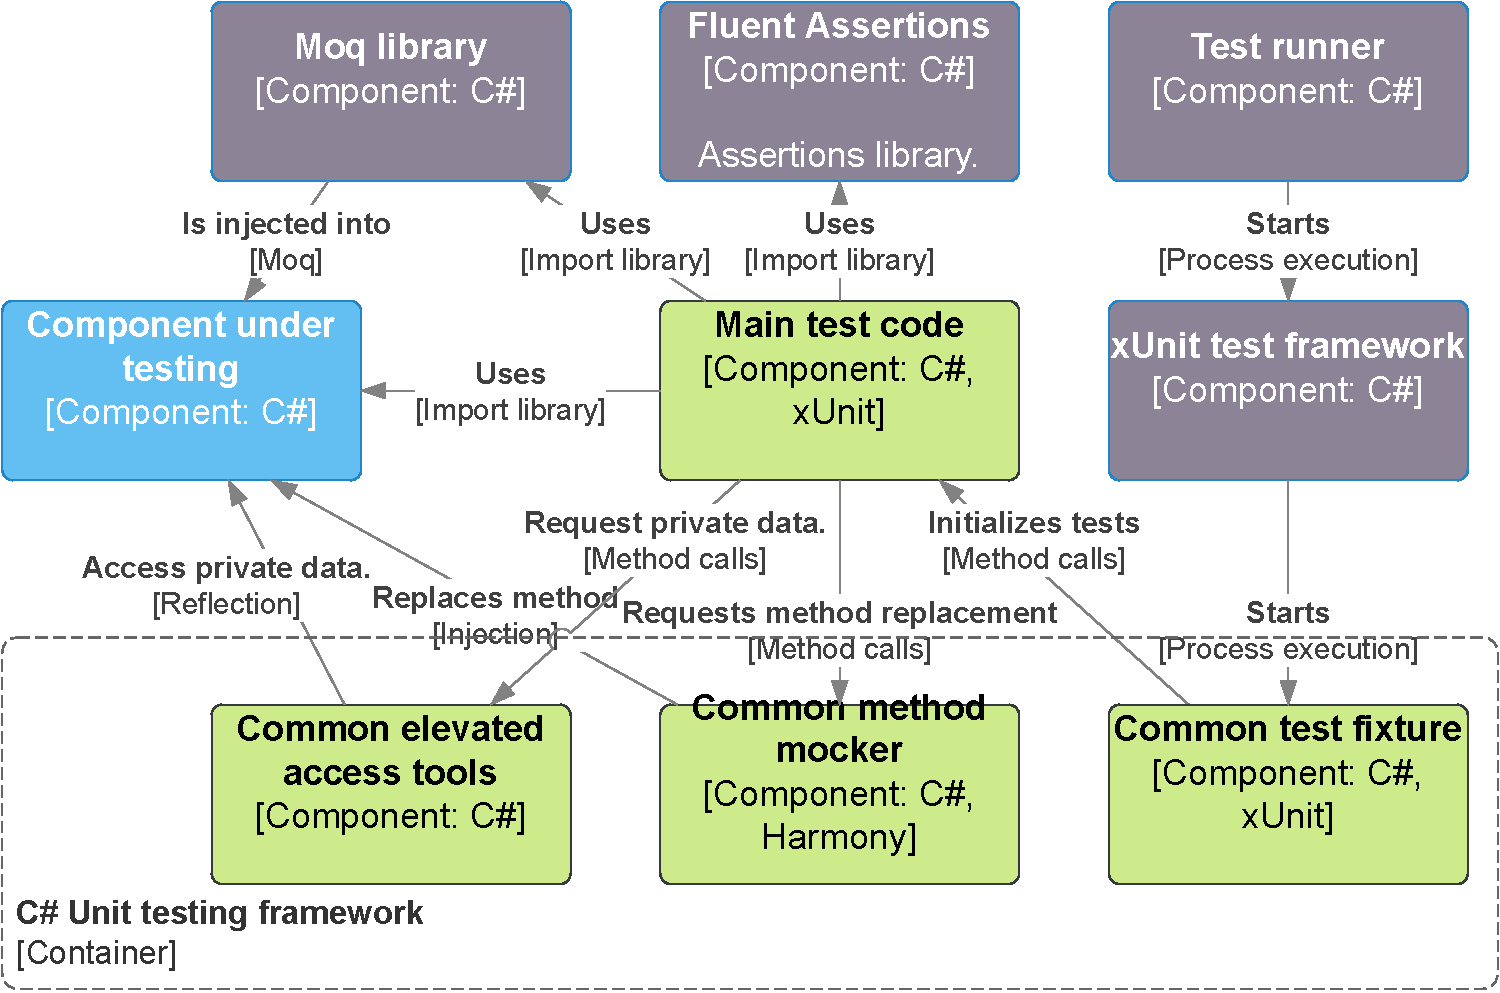
\includegraphics{Backend_unit_testing_component_diagram}
	\caption{Backend unit testing component diagram}
	\label{fig:backend_unit_testing_component_diagram}
\end{figure}

Moq-library was also mainly selected because it is currently the most popular mocking library for the C\#-language \cite{moq2022repository}. Also, during the technical evaluation, it was discovered that most common C\# mocking libraries use Castle DynamicProxy under the hood. Because of that, in the end, they have similar features and limitations. Due to the same backend technology, selecting any mocking library over another has no significant pros or cons.

The fluent Assertions assertion library was also selected mainly due to its popularity. Additionally, Fluent Assertions supported custom error messages, which was mandated by the requirement stated in the \autoref{subsection:test_automation_conventions}. Support for custom error messages was non-existent in the xUnit's build-in assertions library, and because of that build-in assertions library could not be used.

In addition to externally developed libraries, two small testing libraries were internally developed to aid the mocking process. Even though the Moq is a powerful mocking library, it cannot deal with the most complex mocking scenarios and is, for example, unable to interfere with the private class members. In this particular case, some more advanced mocking was required.

The first of the two libraries, "Elevated access tools", provides a convenient wrapper for the C\# reflection in the form of an extension method and enables easy access to private class members. Via the library, developers can easily access, modify or call any private member of the class. The tool was developed because, in some cases, access to private members was seen as advantageous, and no appropriate existing free tools were available.

The second tool, "Method mocker", was developed to address mocking scenarios Moq library could not address. Method mocker can address even the most complex scenarios because it uses dynamic compilation and runtime method replacing, unlike the Moq library that relies on object proxying. Even though the method mocker is more potent than Moq, its disadvantage is that it is slower than Moq due to its dynamic compilation requirements. Because of that, it is only an excellent extension to Moq instead of a replacement for it.

The situation with the frontend unit testing was different compared to the backend unit testing. As seen from the \autoref{fig:frontend_unit_testing_component_diagram}, unlike the backend unit testing architecture, the frontend unit testing architecture does not have many components. There are three primary reasons for this. Because the frontend is written in TypeScript language that compiles into interpreted JavaScript, runtime modification is inherently simple, and additionally, mocking is easy. Secondly, mocking is less often needed in the frontend code because there are, for example, no calls to a database that would always require mocking. Finally, the Angular frontend framework already has an extensive built-in unit testing framework, so there was no need for extensive additional tooling \cite{angular2022testing}. Due to mentioned reasons, the simpler architecture seen in the \autoref{fig:frontend_unit_testing_component_diagram} was selected, consisting mainly of grey external components with one internally developed test component coloured in green and component under testing marked with blue.

\begin{figure}
	\centering
	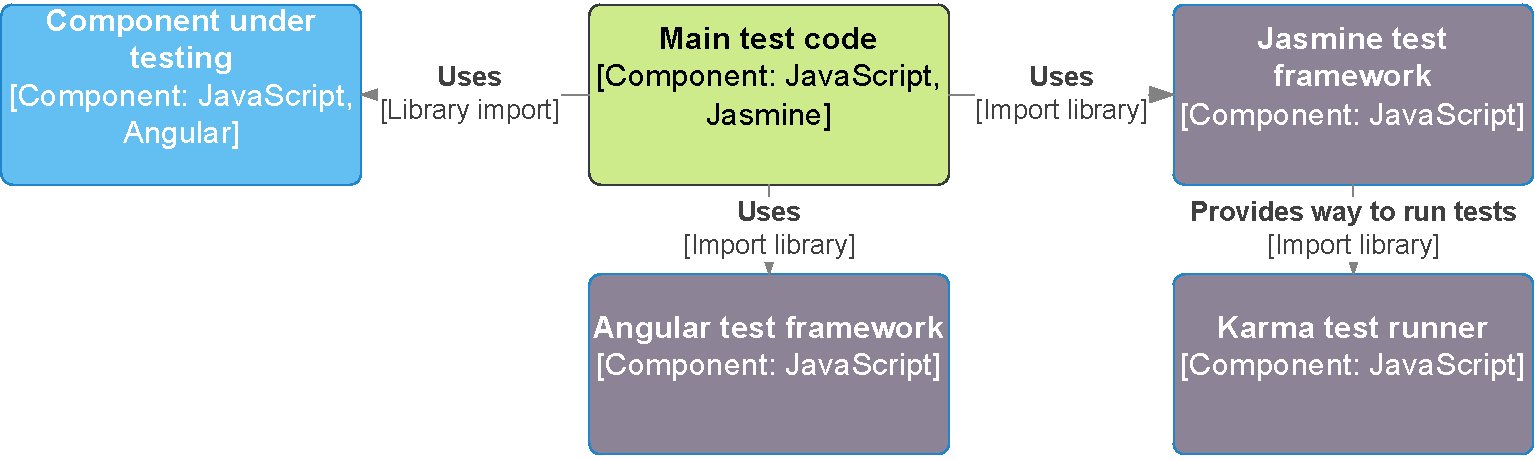
\includegraphics{Frontend_unit_testing_component_diagram}
	\caption{Frontend unit testing component diagram}
	\label{fig:frontend_unit_testing_component_diagram}
\end{figure}

\FloatBarrier

\subsection{Integration test automation}\label{subsection:integration_test_automation}
As mentioned earlier in the \autoref{subsection:integration_testing_architecture}, integration test automation consists of two different integration test automation systems, component and \gls{api} integration test automation. The core of the integration testing architecture is to provide a shared generic platform for installing Hubshare's application and setting up its database automatically. By achieving these goals, a single core framework can support both integration testing frameworks and system-level test automation.

Hubshare's application setup works using a combination of automated file copying, registry and configuration population and, finally, starting up the server process. Setupping the database is more involved. Because it is a valuable feature for the test cases to be able to reset the database state easily to avoid problems with the state entanglement, the database must be set up so that its state can be reset swiftly. Additionally, it would be good if the initialisation of the database would be quick so that the parallelisation of the test runs would be fast. These aspects were emphasised due to the requirements listed in the \autoref{appendix:projects_requirements}.

The database initialisation was separated into two phases to fill the previously mentioned requirements. Database tables, stored procedures and default values are created during the first phase. Additionally, the database is populated with the test data. After that, the database is backed up to the file, and the model database is deleted from the server. During the second phase, the database is restored from the backup as often as needed.

The selected workflow has multiple useful properties. Unless there are changes to the test data, first-phase results can be cached and reused in the subsequent runs, which saves time. Additionally, database reset time should be the smallest possible because the full reset can be achieved by simply restoring the backup from the previously created file, which is an operation provided by the \gls{dbms}.

The \gls{api} test flow can be seen in the \autoref{fig:backend_API_testing_sequence_diagram}. The sequence diagram includes two testing entities called "test" and "test fixture", database, as well as two entities for Hubshare's backend ", Web application" and "Background worker" The sequence starts with the application configuration preparations. After that, the database is initialised. Depending on the situation, this initialisation may include both database initialisation phases or just the second phase if the first phase has already been completed beforehand. Finally, both Hubshare processes are started at the end of the initialisation.

During the testing phase, normal \glsfirst{aaa} pattern is followed, and test-specific preparations, execution and assertions are made. After the test is completed, the database can be restored to its initial state. Revert is done if the test requires it. These steps are repeated for all of the test cases. After all the test cases have been completed, the initialisation process will be reverted, and the setup done during the initialisation phase will be rolled back.

Overall, the component integration testing setup is similar to the \gls{api} integration testing. The main difference is that instead of targeting the \gls{api} endpoints, component integration tests will target the methods inside the application. Component integration tests can also access tools available for backend unit tests, as was presented in the \autoref{fig:test_automation_layers} to test internal methods more efficiently. Regardless of the differences, the core framework code will remain the same for both testing frameworks.

\begin{figure}
	\centering
	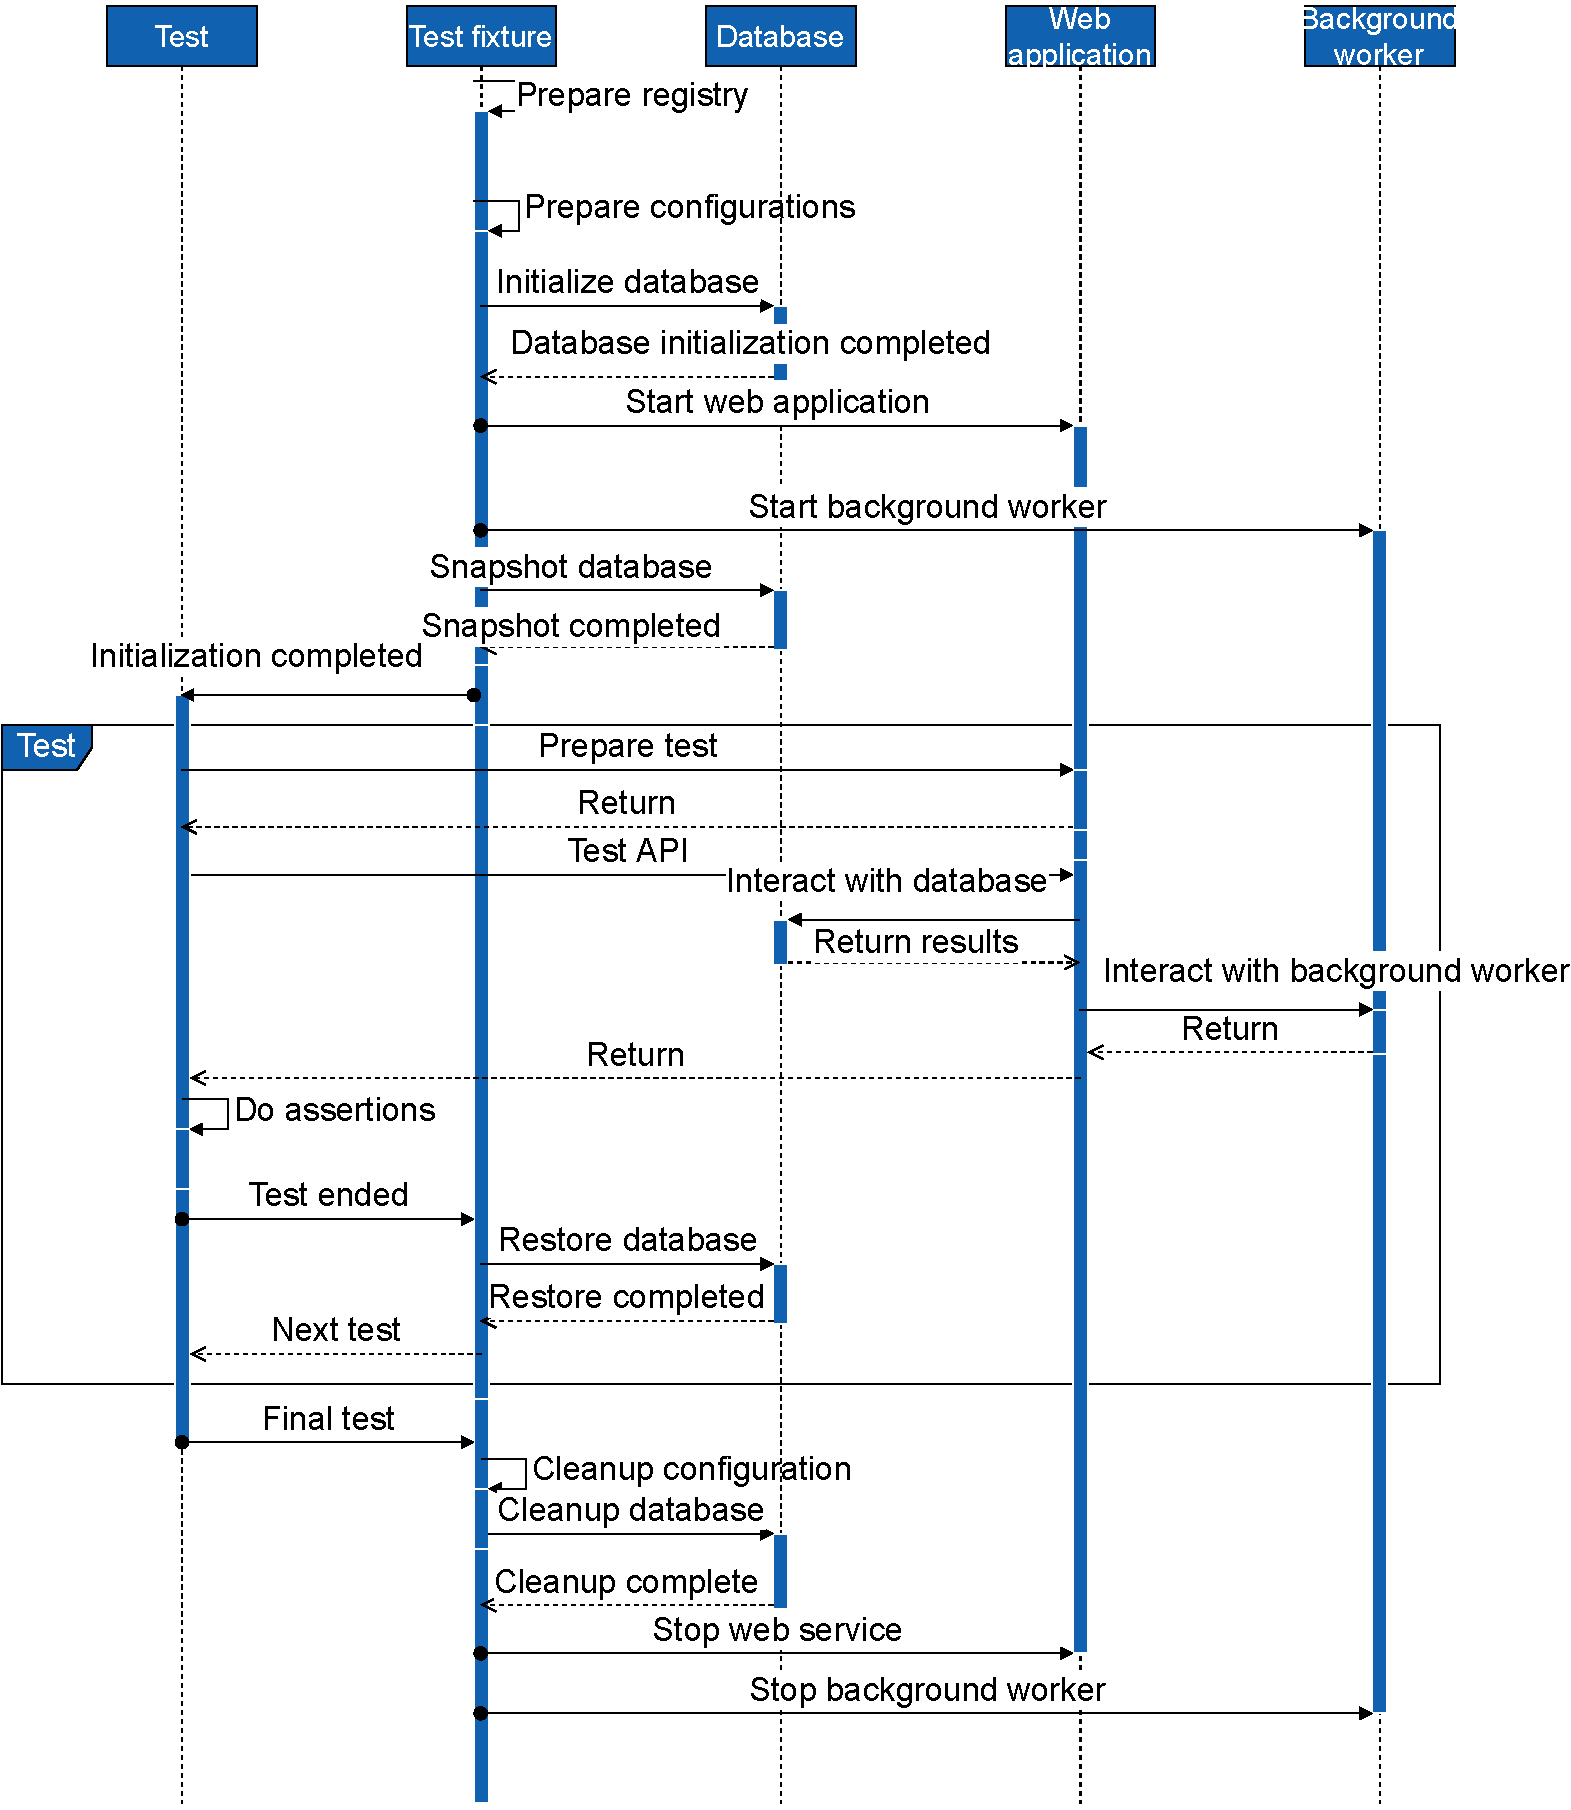
\includegraphics[width=0.9\textwidth]{Backend_API_testing_sequence_diagram}
	\caption{Backend \gls{api} testing sequence diagram}
	\label{fig:backend_API_testing_sequence_diagram}
\end{figure}

\FloatBarrier

\subsection{System test automation}
As quickly mentioned in the \autoref{subsection:integration_test_automation}, system test automation is also based on the integration test automation technologies. In the system testing component diagram, \autoref{fig:system_testing_container_diagram}, this can be seen as "Integration testing framework". If looked closely, the integration testing framework fully manages the whole lower part of the picture. The system testing framework is just an add-on to the other testing layers. Internally developed testing components are coloured in light blue, the internally developed external system is coloured in the dark blue, and externally developed components and containers are coloured in grey.

The definite system-level testing framework consists of two components: the \glsfirst{bdd} interpreter executor and the page model. \gls{bdd} interpreter is a component that interprets the clauses written in the Gherkin's syntax into the logic that the test automation system can execute. This setup is beneficial because the Gherkin's syntax reminds its users of the natural English language and can be understood by anyone if needed. After the interpretation, the interpreter calls appropriate page model functions that map interpreter intents into an appropriate mouse and keyboard events. Additionally page model keeps track of the application state so that the state can be asserted. Page model is helpful because it abstracts the direct \gls{ui} manipulation logic away from the interpreter simplifying its design.

\begin{figure}
	\centering
	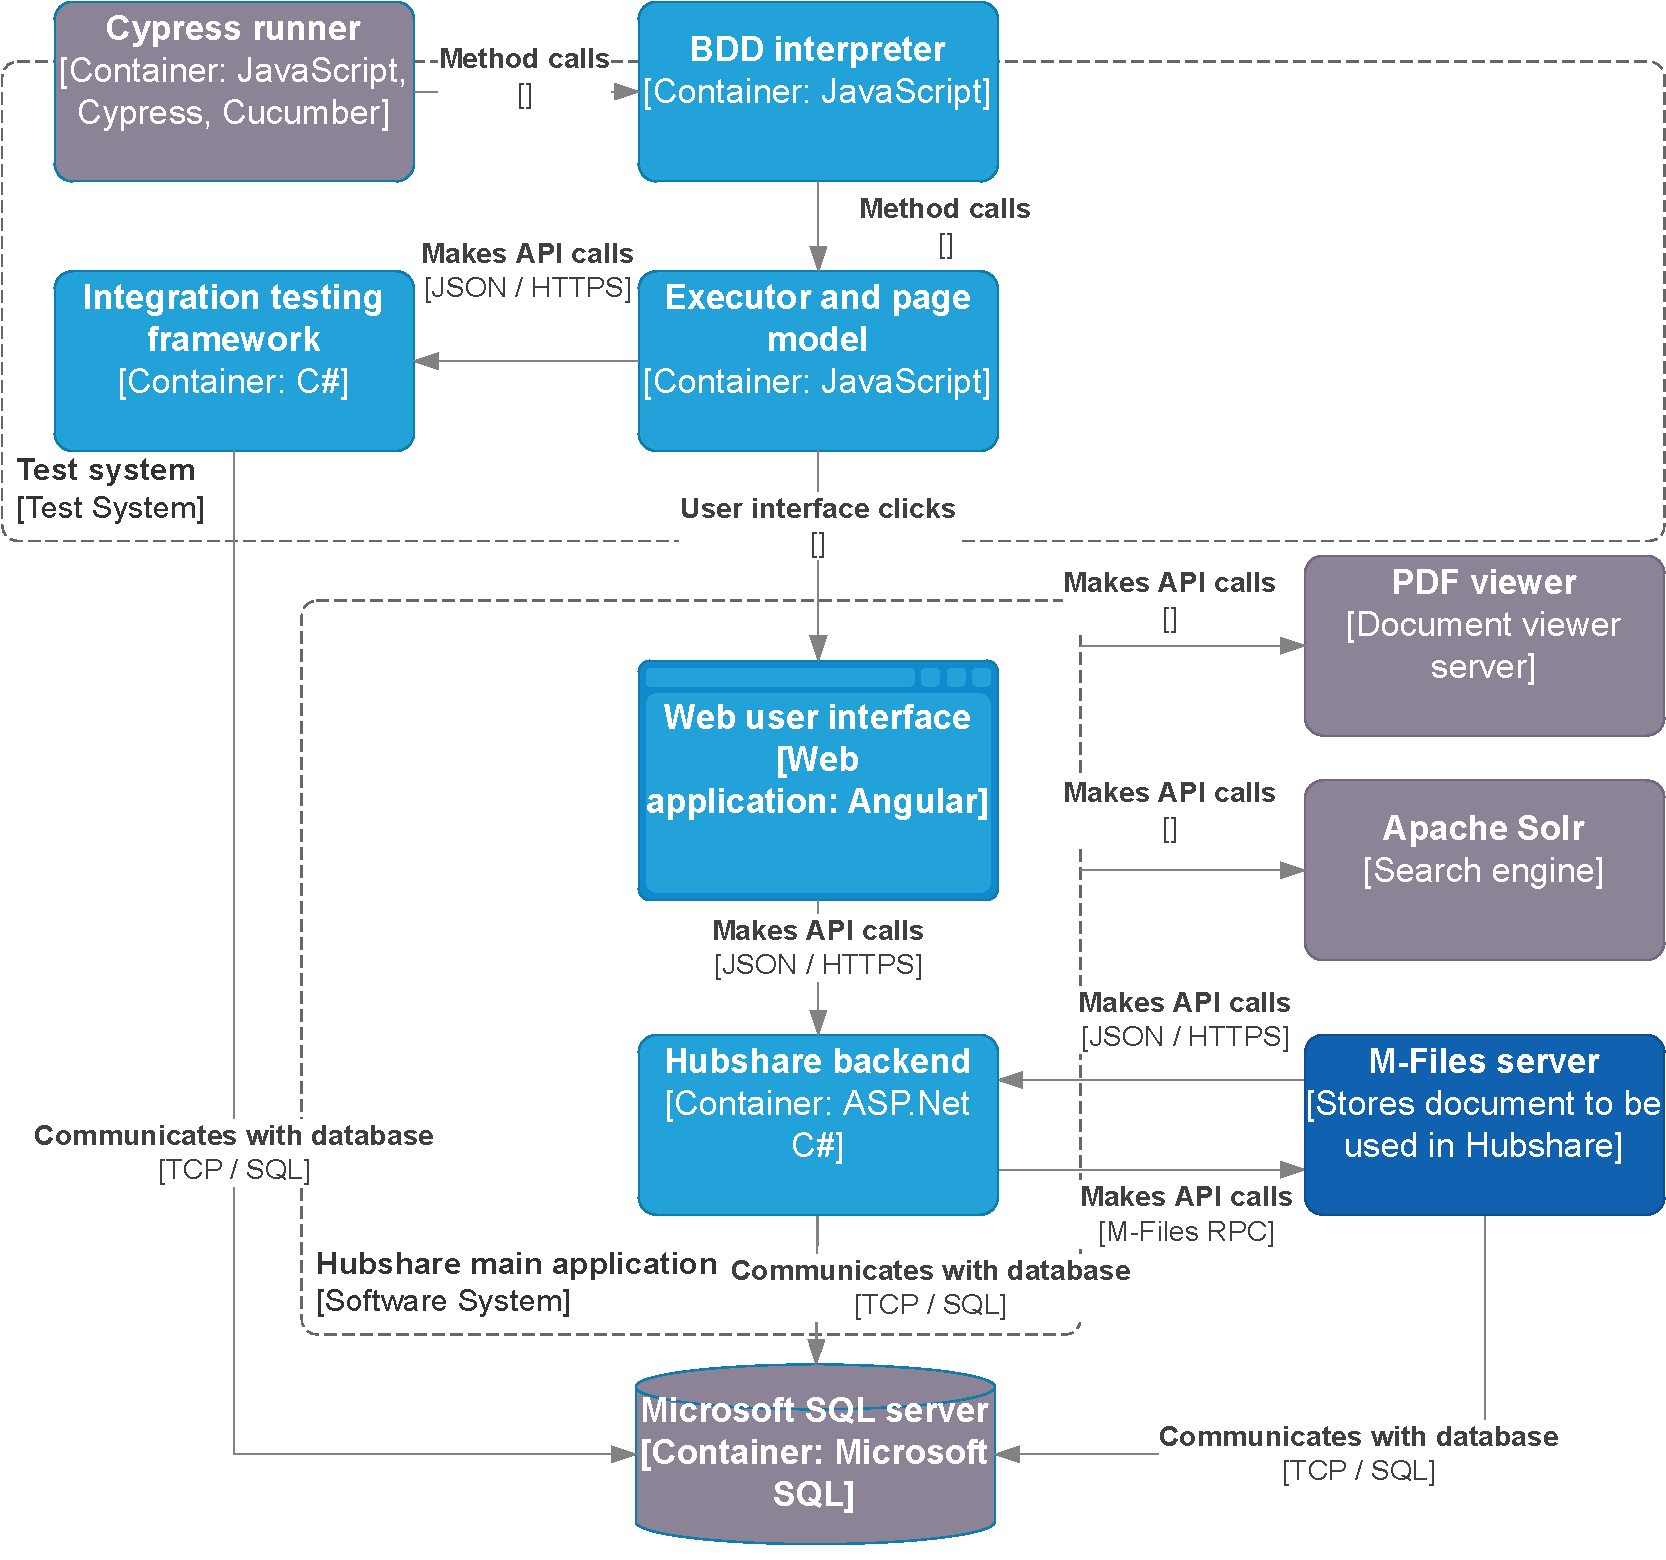
\includegraphics[width=0.95\textwidth]{System_testing_container_diagram}
	\caption{System testing container / component diagram}
	\label{fig:system_testing_container_diagram}
\end{figure}